\newpage
\subsection{Lukket kabinet}
Der blev først og fremmest set på karakteristikken for et helt lukket kabinet. Det vil altså sige, at alle propper blev sat over basreflekshullerne. Frekvenskarakteristikken blev herefter målt med CLIO Pocket lige foran membranen og i \SI{1}{\meter} afstand foran membranen. Resultatet af disse målinger ses på figuren nedenfor.
\begin{figure}[H]
	\centering
	\vspace{-12pt}
	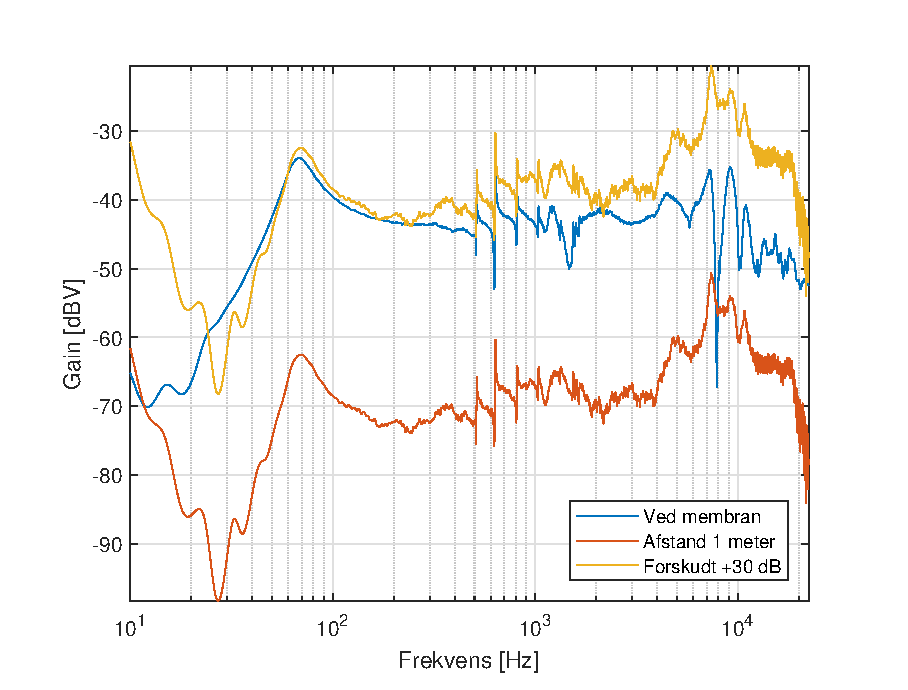
\includegraphics[width=\textwidth]{Billeder/Grafer/ClosedCabinet}
	\caption{Målinger på et lukket kabinet}
\end{figure}

Disse måleresultater udtaler sig som sagt ikke om hvordan basrefleksen påvirker frekvenskarakteristikken - men de vil blive brugt som referencemålinger i mange af de følgende måleopstillinger og resultater.

\begin{wrapfigure}{r}{0.5\textwidth} 
	\vspace{-20pt}
	\begin{center}
		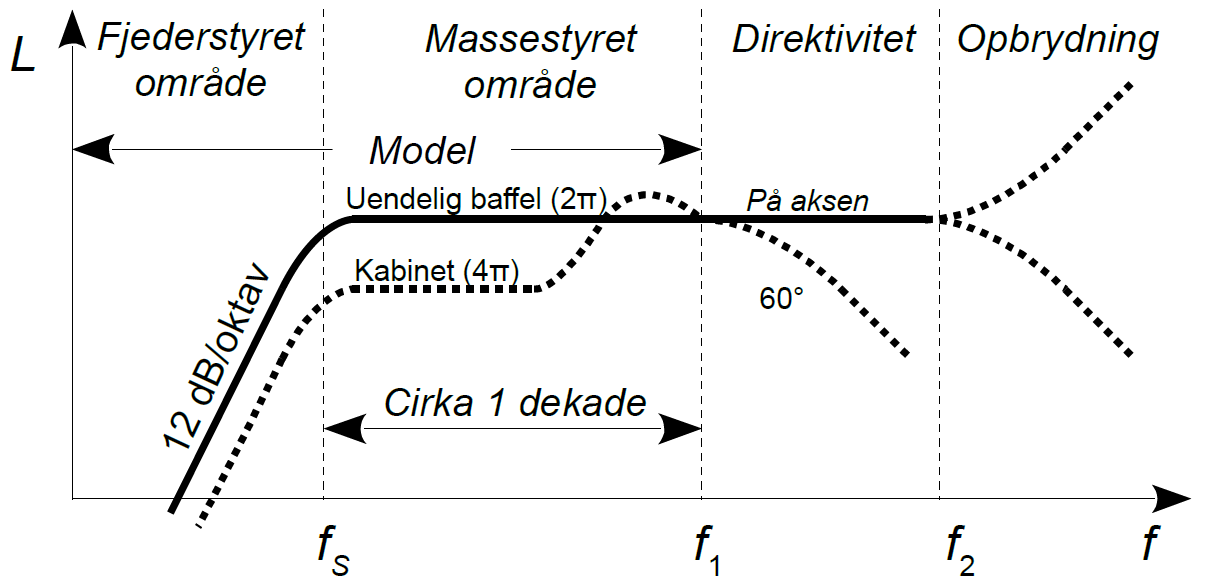
\includegraphics[width=0.5\textwidth]{Billeder/FrekvenskarakteristikTeori}
	\end{center}
	\vspace{-15pt}
	\caption{Teoretisk frekvenskarakteristik}
	\vspace{-20pt}
\end{wrapfigure}
På figuren ovenfor optræder nogenlunde den type karakteristik vi forventer. Det er især resonansfrekvensen $f_s$ ved \SI{70}{\hertz} som er meget interessant idet denne frekvens adskiller det \textbf{fjederstyrede område} fra det \textbf{massestyrede område}. Derudover er der blevet målt en hældning på kurven svarende til omkring +18 dB/oktav i det fjederstyrede område - altså en smule mere end den teoretiske stigning på 12 dB/oktav.

\newpage
For at kunne sammenholde de målte data med vores simulerede data, så er der blevet tilføjet en simuleret kurve på grafen ovenfor. Kurvens placering på Y-aksen er dog arbitrær og vil kun afhænge af forstærkningen i højtaleren. Den simulerede kurve har dog ingen peak ved sin resonansfrekvens - \fxnote{hvorfor har den ikke det? - TS} men den tilsvarende frekvens vil være \SI{-3}{\decibel}-frekvensen som ligger ved \SI{86}{\hertz}; altså \SI{16}{\hertz} over den målte.

På grafen ses det også, at når CLIO-mikrofonen flyttes længere væk fra membranen, så bevarer karakteristikken nogenlunde sin form omkring resonansfrekvensen - men bliver blot dæmpet med omkring \SI{30}{\decibel}. Denne dæmpning er forsøgt vist på grafen (gul)

Ved de laveste frekvenser (under \SI{20}{\hertz}) ligner to former ikke længere hinanden. Dette er dog under det hørbare spektrum og er ikke interessant for disse målinger, men den kan skyldes, at dæmpningsfaktoren i luft er meget anderledes ved lave frekvenser i forhold til høje frekvenser.

På samme måde begynder to grafer at afvige fra hinanden ved frekvenser over \SI{1000}{\hertz}. Dette passer dog fint med, at vi bevæger os ind i et frekvensområde, hvor karakteristikken i større og større grad bliver afhængig af direktiviteten. Det er altså meget muligt, at CLIO-mikrofonen ikke blev placeret præcist lige ud for højtalermembranen.

For at eftervise at de fundne målinger, så ses der på den nedenstående formel; som giver en sammenhæng mellem lydtryk og afstand fra lydgiveren:
\begin{equation}
L_2 = L_1 - \left| 20 \cdot \log \left( \frac{r_1}{r_2} \right) \right|
\end{equation}

Hvor værdierne $L_1$ og $L_2$ er lydtryksniveauet målt i afstandene $r_1$ og $r_2$. Hvis der ses peaken omkring den første resonansfrekvens $f_s$, så ligger denne ved omkring $-\SI{34}{\decibel}$ når der måles tæt på højtaleren og $-\SI{62.5}{\decibel}$, når der måles i 1 meters afstand. Hvis disse værdier indsættes i den førnævnte formel, så findes der følgende:
\begin{equation}
\SI{-62.5}{\decibel} = \SI{-34}{\decibel} - \left| 20 \cdot \log \left( \frac{r_1}{\SI{1.00}{\meter}} \right)\right| \quad \Rightarrow \quad r_1 \approxeq \SI{3}{\centi\meter}
\end{equation}

Hvilket altså vil sige, at CLIO-mikrofonen har været placeret omkring \SI{3}{\centi\meter} fra højtaleren. Dette virker også meget sandsynligt.